\documentclass[tikz,border=3pt]{standalone}
\usepackage{mathptmx}
\usepackage{xcolor}
\usetikzlibrary{arrows.meta,calc}
\definecolor{stripcolor}{RGB}{255,247,199}
\definecolor{loopred}{RGB}{190,20,35}
\definecolor{boxline}{RGB}{38,38,38}
\newcommand{\HeaderFont}{\fontsize{9.4}{10.0}\selectfont}
\newcommand{\BodyFont}{\fontsize{8.75}{8.9}\selectfont}
\newcommand{\NoteFont}{\fontsize{8.75}{8.9}\selectfont}
\newcommand{\ClosingFont}{\fontsize{8.75}{9.2}\selectfont}
\newcommand{\emitpt}[3]{%
  \pgfpointanchor{#2}{#3}\pgfgetlastxy{\ptx}{\pty}%
  \typeout{FIGPT #1 \ptx\space\pty}}
\newcommand{\emitnodebox}[2]{%
  \emitpt{#1.sw}{#2}{south west}%
  \emitpt{#1.ne}{#2}{north east}}
\newcommand{\emitrect}[3]{%
  \emitpt{#1.sw}{#2}{center}%
  \emitpt{#1.ne}{#3}{center}}
\begin{document}
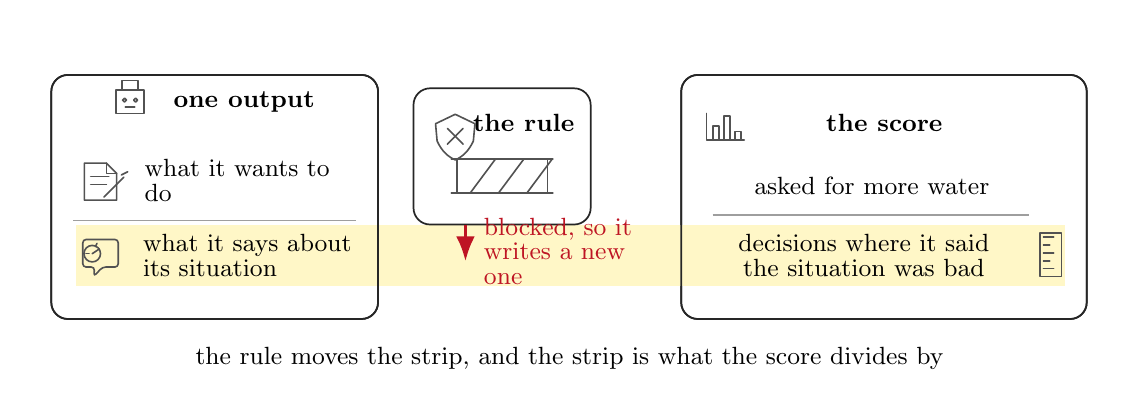
\begin{tikzpicture}[
  >=Latex,
  every node/.style={inner sep=0.8pt},
  header/.style={font=\HeaderFont\bfseries, align=center},
  body/.style={font=\BodyFont, align=center},
  note/.style={font=\NoteFont, align=left},
  closing/.style={font=\ClosingFont, align=center},
  box/.style={rounded corners=6pt, line width=0.62pt, draw=boxline, fill=white},
  fine/.style={line width=0.42pt, draw=black!38},
  icon/.style={line width=0.58pt, draw=black!68, line cap=round, line join=round},
  redarrow/.style={->, line width=1.35pt, draw=loopred}
]
\path[use as bounding box] (0,0) rectangle (13.75,4.55);
\coordinate (canvasSW) at (0,0);
\coordinate (canvasNE) at (13.75,4.55);

\coordinate (outputSW) at (0.30,0.85);
\coordinate (outputNE) at (4.45,3.95);
\coordinate (ruleSW) at (4.90,2.05);
\coordinate (ruleNE) at (7.15,3.78);
\coordinate (scoreSW) at (8.30,0.85);
\coordinate (scoreNE) at (13.45,3.95);
\coordinate (stripSW) at (0.62,1.27);
\coordinate (stripNE) at (13.18,2.05);
\coordinate (rowwantsSW) at (0.55,2.31);
\coordinate (rowwantsNE) at (4.22,2.91);
\coordinate (rednoteSW) at (5.68,1.34);
\coordinate (rednoteNE) at (8.02,2.07);
\coordinate (fracnumSW) at (8.72,2.30);
\coordinate (fracnumNE) at (12.72,2.78);
\coordinate (closingSW) at (0.30,0.08);
\coordinate (closingNE) at (13.45,0.62);

\filldraw[box] (outputSW) rectangle (outputNE);
\filldraw[box] (scoreSW) rectangle (scoreNE);
\fill[stripcolor] (stripSW) rectangle (stripNE);
\filldraw[box] (ruleSW) rectangle (ruleNE);
\draw[box, fill opacity=0, draw opacity=1] (outputSW) rectangle (outputNE);
\draw[box, fill opacity=0, draw opacity=1] (scoreSW) rectangle (scoreNE);
\draw[fine] (0.58,2.10) -- (4.17,2.10);
\draw[fine] (8.70,2.17) -- (12.72,2.17);

% Output icon and label.
\draw[icon] (1.12,3.46) rectangle (1.48,3.76);
\draw[icon] (1.20,3.76) -- (1.20,3.88) -- (1.40,3.88) -- (1.40,3.76);
\draw[icon] (1.23,3.63) circle (0.025);
\draw[icon] (1.37,3.63) circle (0.025);
\draw[icon] (1.24,3.54) -- (1.36,3.54);
\node[header] (txtoneoutput) at (2.75,3.61) {one output};

% Action row.
\draw[icon] (0.72,2.36) -- (0.72,2.83) -- (1.00,2.83) -- (1.13,2.70) -- (1.13,2.36) -- cycle;
\draw[icon] (1.00,2.83) -- (1.00,2.70) -- (1.13,2.70);
\draw[icon] (0.80,2.66) -- (1.03,2.66);
\draw[icon] (0.80,2.56) -- (1.00,2.56);
\draw[icon] (0.97,2.40) -- (1.22,2.65);
\draw[icon] (1.19,2.68) -- (1.27,2.72);
\node[body, anchor=west, align=left, text width=2.55cm] (txtwants) at (1.45,2.61)
  {what it wants to do};

% Situation row: the continuous strip begins here.
\draw[icon, rounded corners=1.2pt]
  (0.70,1.51) -- (0.70,1.86) -- (1.15,1.86) -- (1.15,1.51) -- (0.95,1.51)
  -- (0.84,1.39) -- (0.85,1.51) -- cycle;
\draw[icon] (0.82,1.68) circle (0.105);
\draw[icon] (0.82,1.68) -- (0.91,1.74);
\draw[icon] (0.74,1.68) -- (0.78,1.68);
\draw[icon] (0.86,1.77) -- (0.88,1.81);
\node[body, anchor=west, align=left, text width=2.72cm] (txtsituation) at (1.43,1.66)
  {what it says about its situation};

% Rule box on the strip.
\draw[icon] (5.18,3.33) -- (5.43,3.45) -- (5.68,3.33) -- (5.66,3.11)
  .. controls (5.60,2.98) and (5.52,2.91) .. (5.43,2.87)
  .. controls (5.34,2.91) and (5.26,2.98) .. (5.20,3.11) -- cycle;
\draw[icon] (5.33,3.27) -- (5.53,3.07);
\draw[icon] (5.53,3.27) -- (5.33,3.07);
\node[header] (txtruleheader) at (6.30,3.34) {the rule};
\draw[icon] (5.45,2.45) -- (5.45,2.88);
\draw[icon] (6.60,2.45) -- (6.60,2.88);
\draw[icon] (5.38,2.45) -- (6.67,2.45);
\draw[icon] (5.38,2.88) -- (6.67,2.88);
\draw[icon] (5.62,2.45) -- (5.94,2.88);
\draw[icon] (5.98,2.45) -- (6.30,2.88);
\draw[icon] (6.34,2.45) -- (6.66,2.88);
\draw[redarrow] (5.56,2.05) -- (5.56,1.58);
\node[note, text=loopred, anchor=west, text width=2.18cm] (txtblocked) at (5.76,1.71)
  {blocked, so it writes a new one};

% Score box and denominator endpoint.
\draw[icon] (8.62,3.46) -- (8.62,3.12) -- (9.10,3.12);
\draw[icon] (8.70,3.12) rectangle (8.78,3.30);
\draw[icon] (8.84,3.12) rectangle (8.92,3.43);
\draw[icon] (8.98,3.12) rectangle (9.06,3.23);
\node[header] (txtscoreheader) at (10.88,3.34) {the score};
\node[body] (txtnumerator) at (10.72,2.54) {asked for more water};
\node[body, text width=4.10cm] (txtdenominator) at (10.62,1.66)
  {decisions where it said the situation was bad};
\draw[icon] (12.86,1.39) rectangle (13.13,1.94);
\draw[icon] (12.90,1.89) -- (13.03,1.89);
\draw[icon] (12.90,1.79) -- (12.98,1.79);
\draw[icon] (12.90,1.69) -- (13.03,1.69);
\draw[icon] (12.90,1.59) -- (12.98,1.59);
\draw[icon] (12.90,1.49) -- (13.03,1.49);

\node[closing] (txtclosing) at (6.88,0.35)
  {the rule moves the strip, and the strip is what the score divides by};

\emitrect{canvas}{canvasSW}{canvasNE}
\emitnodebox{txt_one_output}{txtoneoutput}
\emitnodebox{txt_wants}{txtwants}
\emitnodebox{txt_situation}{txtsituation}
\emitnodebox{txt_rule_header}{txtruleheader}
\emitnodebox{txt_blocked}{txtblocked}
\emitnodebox{txt_score_header}{txtscoreheader}
\emitnodebox{txt_numerator}{txtnumerator}
\emitnodebox{txt_denominator}{txtdenominator}
\emitnodebox{txt_closing}{txtclosing}
\emitrect{box_output}{outputSW}{outputNE}
\emitrect{row_wants}{rowwantsSW}{rowwantsNE}
\emitrect{strip}{stripSW}{stripNE}
\emitrect{box_rule}{ruleSW}{ruleNE}
\emitrect{red_note}{rednoteSW}{rednoteNE}
\emitrect{box_score}{scoreSW}{scoreNE}
\emitrect{frac_num}{fracnumSW}{fracnumNE}
\emitrect{closing_band}{closingSW}{closingNE}
\end{tikzpicture}
\end{document}
